\documentclass{ctexart}
\usepackage{etex}
\usepackage{tikz}
\usepackage{pgfplots}
\usepgfplotslibrary{polar,colormaps,colorbrewer}
\pgfplotsset{compat=1.16}
\usepackage{ctex,metalogo}
\usetikzlibrary{calc,decorations.markings,3d}
\setmainfont{TeX Gyre Pagella}
\usepackage{amssymb,amsmath,pgfornament,shapepar}
\usetikzlibrary{shapes.geometric,through,decorations.pathmorphing, arrows.meta,quotes,mindmap,shapes.symbols,shapes.arrows,automata,angles,3d,trees,shadows,automata,arrows,
shapes.callouts}
\begin{document}









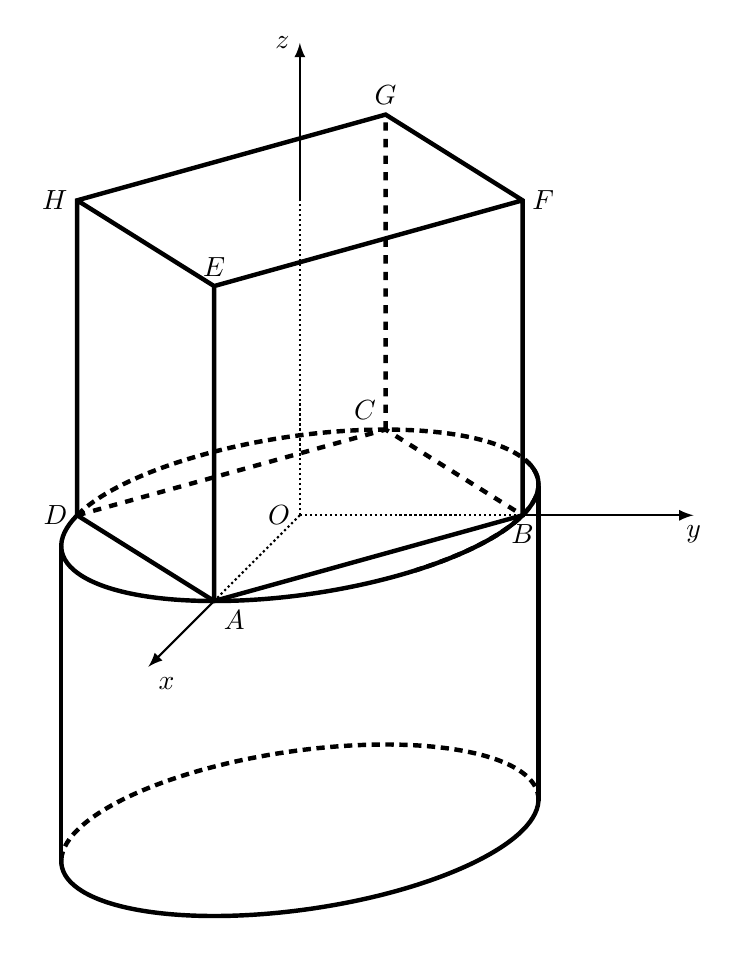
\begin{tikzpicture}
    \coordinate[label=left:$O$] (O) at (0,0,0);
    \coordinate[label=below right:$A$] (A) at (0,0,{2*sqrt(2)});
    \coordinate[label=below:$B$] (B) at ({2*sqrt(2)},0);
    \coordinate[label=above left:$C$] (C) at (0,0,{-2*sqrt(2)});
    \coordinate[label=left:$D$] (D) at ($(A) + (C) - (B)$);
    \coordinate (Z) at (90:4);
    \coordinate[label=above:$E$] (E) at ($(A) + (Z)$);
    \coordinate[label=right:$F$] (F) at ($(B) + (Z)$);
    \coordinate[label=above:$G$] (G) at ($(C) + (Z)$);
    \coordinate[label=left:$H$] (H) at ($(D) + (Z)$);
    \draw[ultra thick](D)--(A)--(B)--(F)--(G)--(H)--cycle (H)--(E)--(F) (E)--(A);
    \draw[ultra thick, dashed](D)--(C)--(B) (C)--(G);

    \begin{scope}[canvas is xz plane at y=0]
        \draw[ultra thick] (B) arc [start angle=0, end angle = 180, radius={2*sqrt(2)}];
        \draw[ultra thick] (B) arc [start angle=0, end angle = -40, radius={2*sqrt(2)}];
        \draw[ultra thick, densely dashed] (D) arc [start angle=-180, end angle = 40, radius={2*sqrt(2)}];
    \end{scope}

    \begin{scope}[rotate around y=20]
        \begin{scope}[canvas is xz plane at y=-4]
            \draw[ultra thick] ({2*sqrt(2)},0) arc [start angle=0, end angle = 180, radius={2*sqrt(2)}];
            \draw[ultra thick, densely dashed] ({-2*sqrt(2)},0) arc [start angle=-180, end angle = 0, radius={2*sqrt(2)}];
        \end{scope}

        \draw[ultra thick] ({2*sqrt(2)},0)--({2*sqrt(2)},-4);
        \draw[ultra thick] ({-2*sqrt(2)},0)--({-2*sqrt(2)},-4);
    \end{scope}

    \draw[thick, densely dotted](0,0)--(B);
    \draw[->,>=latex,thick](B)--(5,0)node[below]{$y$};
    \draw[thick, densely dotted](0,0)--(0,4);
    \draw[->,>=latex,thick](0,4)--(0,6)node[left]{$z$};
    \draw[thick, densely dotted](0,0)--(A);
    \draw[->,>=latex,thick](A)--(0,0,5)node[below right]{$x$};
\end{tikzpicture}












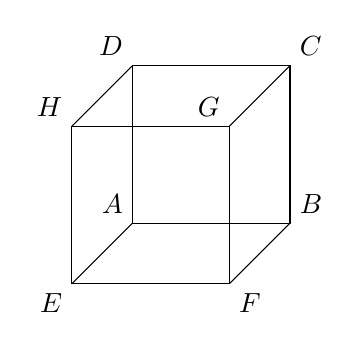
\begin{tikzpicture}[scale=2]
    % 定义立方体的顶点
    \coordinate (A) at (0,0,0);
    \coordinate (B) at (1,0,0);
    \coordinate (C) at (1,1,0);
    \coordinate (D) at (0,1,0);
    \coordinate (E) at (0,0,1);
    \coordinate (F) at (1,0,1);
    \coordinate (G) at (1,1,1);
    \coordinate (H) at (0,1,1);

    % 绘制底面
    \draw (A) -- (B) -- (C) -- (D) -- cycle;
    % 绘制顶面
    \draw (E) -- (F) -- (G) -- (H) -- cycle;
    % 绘制侧面
    \draw (A) -- (E);
    \draw (B) -- (F);
    \draw (C) -- (G);
    \draw (D) -- (H);

    % 标注顶点
    \node[above left] at (A) {$A$};
    \node[above right] at (B) {$B$};
    \node[above right] at (C) {$C$};
    \node[above left] at (D) {$D$};
    \node[below left] at (E) {$E$};
    \node[below right] at (F) {$F$};
    \node[above left] at (G) {$G$};
    \node[above left] at (H) {$H$};
\end{tikzpicture}















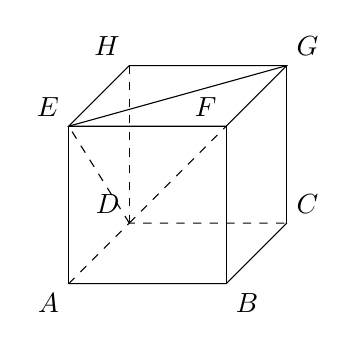
\begin{tikzpicture}[scale=2]
    % 定义立方体的顶点
    \coordinate (A) at (0,0,1);
    \coordinate (B) at (1,0,1);
    \coordinate (C) at (1,0,0);
    \coordinate (D) at (0,0,0);
    \coordinate (H) at (0,1,0);
    \coordinate (G) at (1,1,0);
    \coordinate (F) at (1,1,1);
    \coordinate (E) at (0,1,1);
    % 绘制底面
    \draw (A) -- (B) -- (C);
    \draw[dashed]  (A) -- (D) -- (C);
    % 绘制顶面
    \draw (E) -- (F) -- (G) -- (H) -- cycle;
    % 绘制侧面
    \draw (A) -- (E);
    \draw[dashed] (D) -- (H);
    \draw[dashed] (D) -- (F);
    \draw[dashed] (D) -- (E);
    \draw (G) -- (E);
    \draw (B) -- (F);
    \draw (C) -- (G);
    % 标注顶点
    \node[below left] at (A) {$A$};
    \node[below right] at (B) {$B$};
    \node[above right] at (C) {$C$};
    \node[above left] at (D) {$D$};
    \node[above left] at (E) {$E$};
    \node[above left] at (F) {$F$};
    \node[above right] at (G) {$G$};
    \node[above left] at (H) {$H$};
\end{tikzpicture}
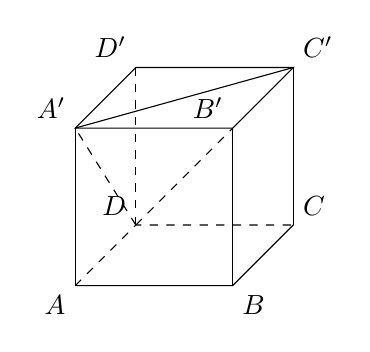
\begin{tikzpicture}[scale=2]
    % 定义立方体的顶点
    \coordinate (A) at (0,0,1);
    \coordinate (B) at (1,0,1);
    \coordinate (C) at (1,0,0);
    \coordinate (D) at (0,0,0);
    \coordinate (H) at (0,1,0);
    \coordinate (G) at (1,1,0);
    \coordinate (F) at (1,1,1);
    \coordinate (E) at (0,1,1);
    % 绘制底面
    \draw (A) -- (B) -- (C);
    \draw[dashed]  (A) -- (D) -- (C);
    % 绘制顶面
    \draw (E) -- (F) -- (G) -- (H) -- cycle;
    % 绘制侧面
    \draw (A) -- (E);
    \draw[dashed] (D) -- (H);
    \draw[dashed] (D) -- (F);
    \draw[dashed] (D) -- (E);
    \draw (G) -- (E);
    \draw (B) -- (F);
    \draw (C) -- (G);
    % 标注顶点
    \node[below left] at (A) {$A$};
    \node[below right] at (B) {$B$};
    \node[above right] at (C) {$C$};
    \node[above left] at (D) {$D$};
    \node[above left] at (E) {$A'$};
    \node[above left] at (F) {$B'$};
    \node[above right] at (G) {$C'$};
    \node[above left] at (H) {$D'$};
\end{tikzpicture}


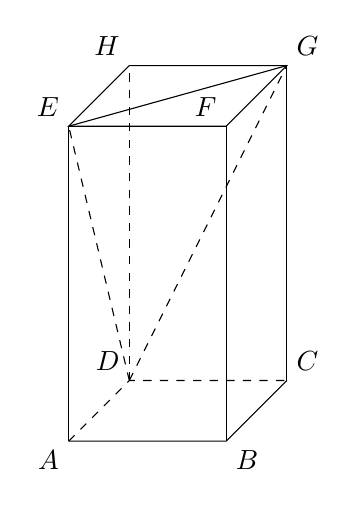
\begin{tikzpicture}[scale=2]
    % 定义立方体的顶点
    \coordinate (A) at (0,0,1);
    \coordinate (B) at (1,0,1);
    \coordinate (C) at (1,0,0);
    \coordinate (D) at (0,0,0);
    \coordinate (H) at (0,2,0);
    \coordinate (G) at (1,2,0);
    \coordinate (F) at (1,2,1);
    \coordinate (E) at (0,2,1);
    % 绘制底面
    \draw (A) -- (B) -- (C);
    \draw[dashed]  (A) -- (D) -- (C);
    % 绘制顶面
    \draw (E) -- (F) -- (G) -- (H) -- cycle;
    % 绘制侧面
    \draw (A) -- (E);
    \draw[dashed] (D) -- (H);
    \draw[dashed] (D) -- (G);
    \draw[dashed] (D) -- (E);
    \draw (G) -- (E);
    \draw (B) -- (F);
    \draw (C) -- (G);
    % 标注顶点
    \node[below left] at (A) {$A$};
    \node[below right] at (B) {$B$};
    \node[above right] at (C) {$C$};
    \node[above left] at (D) {$D$};
    \node[above left] at (E) {$E$};
    \node[above left] at (F) {$F$};
    \node[above right] at (G) {$G$};
    \node[above left] at (H) {$H$};
\end{tikzpicture}




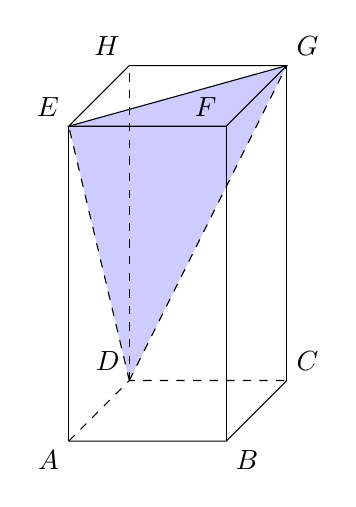
\begin{tikzpicture}[scale=2]
    % 定义立方体的顶点
    \coordinate (A) at (0,0,1);
    \coordinate (B) at (1,0,1);
    \coordinate (C) at (1,0,0);
    \coordinate (D) at (0,0,0);
    \coordinate (H) at (0,2,0);
    \coordinate (G) at (1,2,0);
    \coordinate (F) at (1,2,1);
    \coordinate (E) at (0,2,1);
    % 平面涂色
    \fill[blue!20] (D) -- (G) -- (E) -- cycle;
    % 绘制底面
    \draw (A) -- (B) -- (C);
    \draw[dashed]  (A) -- (D) -- (C);
    % 绘制顶面
    \draw (E) -- (F) -- (G) -- (H) -- cycle;
    % 绘制侧面
    \draw (A) -- (E);
    \draw[dashed] (D) -- (H);
    \draw[dashed] (D) -- (G);
    \draw[dashed] (D) -- (E);
    \draw (G) -- (E);
    \draw (B) -- (F);
    \draw (C) -- (G);
    % 标注顶点
    \node[below left] at (A) {$A$};
    \node[below right] at (B) {$B$};
    \node[above right] at (C) {$C$};
    \node[above left] at (D) {$D$};
    \node[above left] at (E) {$E$};
    \node[above left] at (F) {$F$};
    \node[above right] at (G) {$G$};
    \node[above left] at (H) {$H$};
\end{tikzpicture}






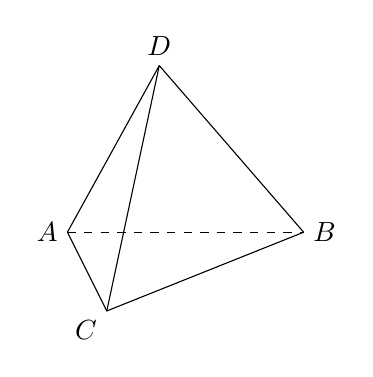
\begin{tikzpicture}[scale = 3]
    % 定义正四面体的顶点坐标
    \coordinate (A) at (0,0,0);%第一个坐标是横的,第二个坐标是往上走,而第三个坐标往纸面外走
    \coordinate (B) at (1,0,0); 
    \coordinate (C) at (0.5, 0,{sqrt(3)/2});
    \coordinate (D) at (0.5,{sqrt(6)/3} , {sqrt(3)/6});

    % 绘制正四面体的边
    \draw (A) -- (C) -- (B);
    \draw[dashed] (A) -- (B);
    \draw (A) -- (D);
    \draw (B) -- (D);
    \draw (C) -- (D);
    \node[ left] at (A) {$A$};
    \node[right ] at (B) {$B$};
    \node[below left] at (C) {$C$};
    \node[above ] at (D) {$D$};

\end{tikzpicture}



\end{document} 